\documentclass[xcolor ={table,usenames,dvipsnames}]{beamer}
\usepackage[italian]{babel}
\usepackage{color}
\usepackage{txfonts}
\PassOptionsToPackage{dvipsnames}{xcolor}
\title{Duck Typing in Python}
\author{Author: Tommaso Puccetti}
\institute{Universit\`a  degli Studi di Firenze}
\date{21/12/2018}
%\usepackage{sansmathaccent}
\usetheme{Berlin} 
\useinnertheme{rounded}
\useoutertheme{miniframes} 
\setbeamercovered{dynamic}
\theoremstyle{definition}
\newtheorem{definizione}{Definizione}
\usepackage{tikz}
\usetikzlibrary{arrows}
\usepackage{subfigure}
\usepackage[procnames]{listings}
\usepackage{color}
\usepackage{jlcode}

\definecolor{keywords}{RGB}{255,0,90}
\definecolor{comments}{RGB}{0,0,113}
\definecolor{red}{RGB}{160,0,0}
\definecolor{green}{RGB}{0,150,0}

\lstset{language=Python, 
	backgroundcolor=\color{yellow},
	basicstyle=\fontsize{2}{4}\selectfont\ttfamily\scriptsize, 
	keywordstyle=\color{keywords},
	commentstyle=\color{comments},
	stringstyle=\color{green},
	showstringspaces=false,
	identifierstyle=\color{black},
	procnamekeys={def,class},
}

\begin{document}
	
	\begin{frame}
		\maketitle
			\begin{figure}[h!]
			\centering
			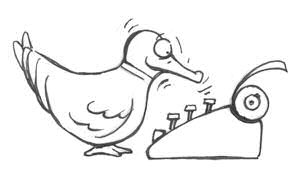
\includegraphics[scale=2]{img/cartoonduck.jpg}
			\label{Interfacce di un CS}
		\end{figure}
	\end{frame}

	\begin{frame}
		\frametitle{Index}
		
	\end{frame}

	\begin{frame}
		\frametitle{Introduction}
		Python is an \textit{\textbf{interpreted}}, \textit{\textbf{multi-paradigm}} language. It was initially designed by Guido van Rossum in 1991 and developed by Python Software Foundation. It supports:
		\begin{itemize}
			\item \textbf{Functional programming } (non pure);
			\item \textbf{Procedural programming};
			\item \textbf{Objected oriented}.
		\end{itemize}
	\end{frame}

	\begin{frame}
		\frametitle{Python's semantic}
			Could be useful to first recall the difference between \textit{\textbf{strict}} and \textit{\textbf{lazy}} evaluation:
			\begin{enumerate}
				\item \textbf{Strict evaluation strategy}: the arguments of a function are fully evaluated to values before evaluating the function call (call by value);
				\item \textbf{Non-strict or Lazy evaluation:} arguments are evaluated only if it is needed in the function body (\textit{call by name})
			\end{enumerate}
			Python:		
			\begin{itemize}
				\item implements \textbf{strict semantic};
				\item uses \textbf{whitespace indentation}, rather than curly brackets or keywords, to delimit blocks.
			\end{itemize}
	\end{frame}

	\begin{frame}[fragile]
		\frametitle{Semantic: Python vs Haskell}
		In Python we never get \textit{true} beacause  it forces the evaluation of the function wich contains an infinite loop in the body:
		\begin{lstlisting}
			def infiniteLoop(x):
			    while True:
		           print("do something with x")
		        return x
				
			5 in [5, 10, infiniteLoop(5)]
		\end{lstlisting}
		If we write the same code in \textbf{haskell} we get the \textit{true} value:
		\begin{lstlisting}
			elem 2 [2, 4, noreturn 5]
		\end{lstlisting}
	\end{frame}

	\begin{frame}
		\frametitle{Type checker (1)}
			\textbf{Type checking} is the process of verifying and enforces the typing rules of a language.
		\begin{enumerate}
			\item \textbf{Dynamic vs. Static}
			\item \textbf{Weak vs. Strong}.
		\end{enumerate}
		
		\begin{figure}[h!]
			\centering
			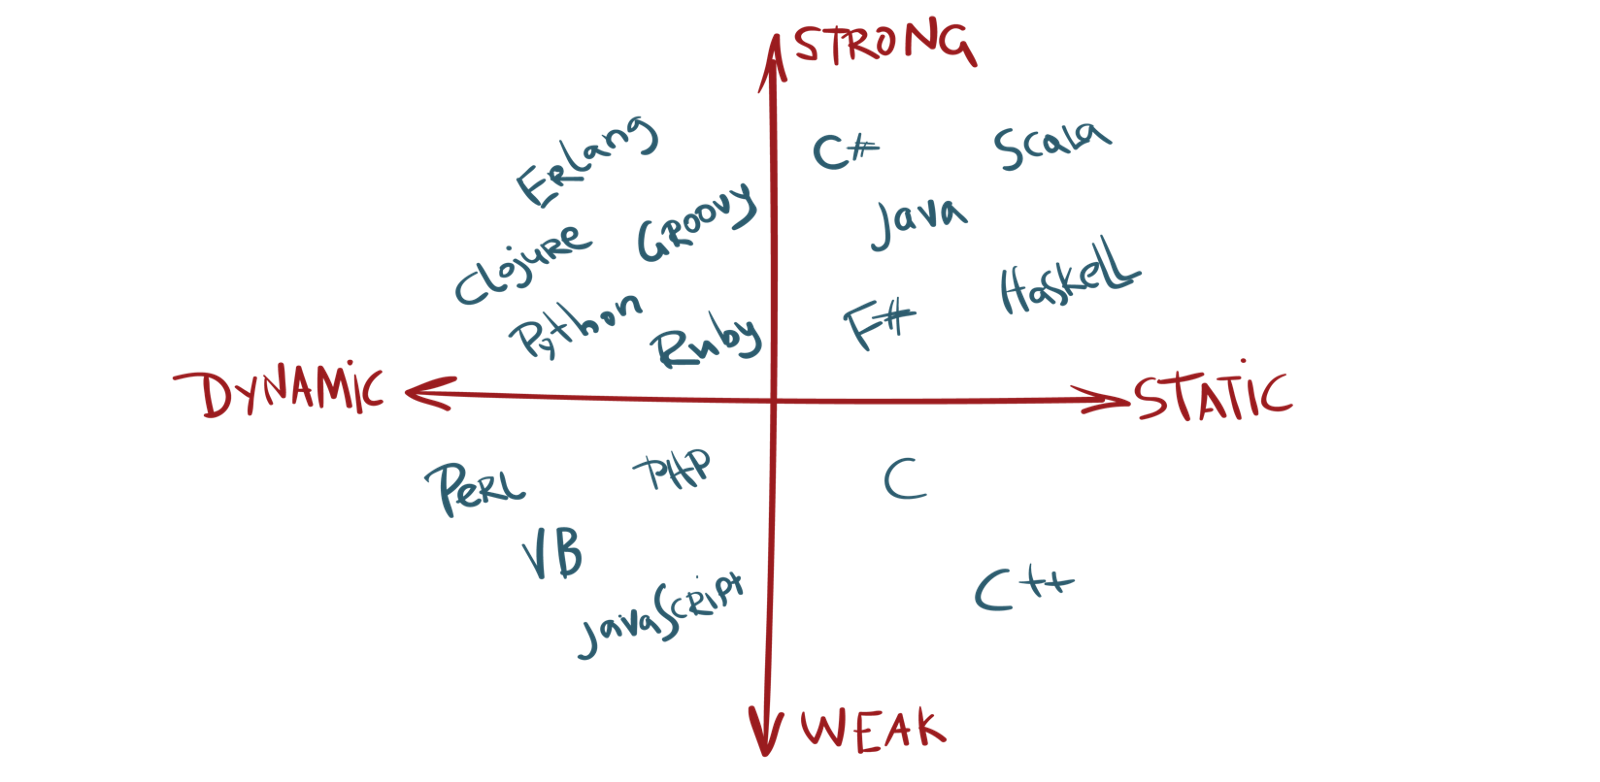
\includegraphics[scale=0.14]{img/classification.png}
		\end{figure}
	\end{frame}

	\begin{frame}
		\frametitle{Type checker (2) }
		\begin{enumerate}
			\item \textbf{Dynamic vs. Static}\begin{itemize}
				\item \textbf{Statically-typed languages}: typechecking is done at
				compile-time, in order to guarantee the absence of run-time (type) errors:
				formal proof of type-safety.
				\item \textbf{Dynamically-typed languages:} dynamic
				type checking is the process of verifying type constraints at runtime,
				during execution.
			\end{itemize}
			\item \textbf{Weak vs. Strong}\begin{itemize}
				\item AGGIUNGERE STRONGLY
				\item AGGIUNGERE WEAKLY	
			\end{itemize}
		\end{enumerate}
	\end{frame}

	\begin{frame}
		\frametitle{Python's type checker}
			\begin{enumerate}
				\item Python is \textbf{dynamic}: 
				\begin{itemize}
					\item objects have a type but it is determined at runtime;
					\item variables are not explicitly typed;
					\item an assignement binds a name to an object and the object could be of any type;
				\end{itemize}
				\item Python is also \textbf{strongly typed}.
			\end{enumerate}
			Let's see the implications by some example.
	\end{frame}

	\begin{frame}[fragile]
		\frametitle{Python's dynamic typing example (1)}
			\begin{lstlisting} 
			if False:
				print(10+"ten") 
			else:
				print(10+10)
			\end{lstlisting}
			The first branch never execute, so the type checking ignore the type incongruency.
			
			If we try to execute \textbf{separately} the first branch, the type check raise a type error:
			
			\begin{lstlisting}
			TypeError: unsupported operand type(s) for +: 'int' and 'str'
			\end{lstlisting}
	\end{frame}

	\begin{frame}[fragile]
		\frametitle{Python's dynamic typing example (2)}
		Another consequnce is that programmers are \textbf{free to bind the same names (variables) to different objects with a different type}. Then the following statements are perfectly legal:
		
		\begin{lstlisting}
		variable = 10
		variable = "ten"
		\end{lstlisting}
		
		So long as you only perform operations valid for the type the interpreter doesn't care what type they actually are. 
	\end{frame}

	\begin{frame}[fragile]
		\frametitle{Python's strong typing example}
		Python is not allowed to perform operations inappropriate to the type of the object: 
		\begin{lstlisting}
		print(10+"ten")
		\end{lstlisting}
		
		In a \textbf{weakly-typed} language, like PHP, the integer is forced to be a string and no type error is raised:
		\begin{lstlisting}
		$temp = "ten"; 
		$temp = $temp + 10; // no error caused
		echo $temp;
		\end{lstlisting}
	The output will be "ten10".
	\end{frame}

	\begin{frame}[fragile]
		\frametitle{Some exceptions (1)}
		There are some operations allowed even in case of type incongruence.\\
		The\textbf{ boolean equivalence} is permitted in Python 2 and 3: 
		
		\begin{lstlisting}
			print("10" == 10)
			print("10" != 10)
		\end{lstlisting}
		Returning:
		\begin{lstlisting}
			False
			True
		\end{lstlisting}
	\end{frame}

	\begin{frame}[fragile]
		\frametitle{Some exceptions (2)}
		In Python 2 "\textit{grather than}" and \textit{"less than"} are permitted:
		
		\begin{lstlisting}
		print("10">10)
		print("10"<10)
		\end{lstlisting}
		
		Returning:
		
		\begin{lstlisting}
		True
		False
		\end{lstlisting}
		
		Python 3 do not allowed to do "\textit{grather than}" and \textit{"less than"} controls like these.\\	
	\end{frame}

	\begin{frame}[fragile]
		\frametitle{Annotations}
			Annotations were introduced in Python 3.0 and are the main way to add type hints to the code. We can annotate both \textbf{function} and \textbf{variable}.
			
			\begin{lstlisting}
				import math
				
				pi: float = 3.142
				
				def circumference(radius: float) -> float:
					return 2 * math.pi * radius
			\end{lstlisting}
			
			Type hints and annotations \textbf{\textit{do not add a real static typechecking}} in native Python so this should not effect the code performance.\\
	\end{frame}

	\begin{frame}
		\frametitle{Annotations: why use it?}
		\textbf{From PEP 484}:\\
		\textit{" <...>using type hints for performance optimizations is left as an exercise for the reader"}.\\
		
		\textbf{Advantages:}
		\begin{itemize}
			\item Type hints help document your code;
			\item Type hints improve IDEs and linters. This allows IDEs to offer better code completion and similar features.
		\end{itemize}
		\textbf{Disadvantages}
		\begin{itemize}
			\item Type hints take developer time and effort to add.
			\item Type hints introduce a slight penalty in start-up time.
		\end{itemize}
	\end{frame}

	\begin{frame}[fragile]
		\frametitle{Object oriented (1)}
	\begin{lstlisting}
		class Duck():
			def __init__(self, name, colour):
				self.name = name
				self.colour = colour
			def quack(self):
				return "Quaaack"
			def fly(self):
				return "The duck is flying"
		
		donald = Duck("Donald","white")
				
		donald.name
		donald.colour
		donald.quack()
		donald.fly()
		\end{lstlisting}
	\end{frame}

	\begin{frame}[fragile]
		\frametitle{Object oriented (2)}
		\begin{itemize}
			\item The first argument of every class method is always a reference to the current instance of the class (\textit{\textbf{self}}).
			\item The \textbf{\textit{self}} world is the equivalent of \textbf{\textit{this}} in \textbf{Java}. However Java do not requires to pass \textit{this} explicitly as a first parameter of a method: it could be used straight in the body of the method.
			\item However self\textbf{ is not a reserved keyword} in Python, is just a strong convention.
		\end{itemize}
		\begin{lstlisting}[basicstyle=\fontsize{2}{4}\selectfont\ttfamily\tiny]
		class Duck():
			def __init__(myself, name, colour):
				myself.name = name
				myself.colour = colour
			def quack(myself):
				return "Quaaack"	
			def fly(myself):
				return "The duck is flying"
		\end{lstlisting}
	\end{frame}

	\begin{frame}[fragile]
		\frametitle{Object oriented (3)}
		In Python \textbf{is not possible to define multiple constructor} for a class, still is possible to define a default value if one is not passed.
		
		\begin{lstlisting}
		class Parrot():
			def __init__(self, name = "Perry"):
				self.name = name
		
		bird1 = Parrot()
		bird2 = Parrot("Jack")
		
		print(bird1.name)
		print(bird2.name)
		\end{lstlisting}
		The output would be:\\
		"Perry"\\
		"Jack"
	\end{frame}

	
		
	
	

	
	
	
	
	
	
	
	
	
	
	
\end{document}